\section{Businesses}
	\subsection{Registration}
	If you want to create a business account for \textit{Soldino} 
	visit the homepage and make sure that the slider in set on "Citizen".\\
	\begin{figure}[H]
		
\includegraphics[width=5cm]{res/images/user_business.png}
		\centering
		\caption{Select "Business" from the slider}
	\end{figure}	
	\noindent Then, insert your business's data in the form. After you have completed 
	all the	fields with your informations press the "Sign up" button. If an 
	entry is not valid (i.e. the email address does not contain a valid 
	domain) the system will let you know and you have to correct that field 
	to continue. If all the informations are correct a pop up window will open 
	asking you to allow \textit{Soldino} to access your information.\\
	\begin{figure}[H]
		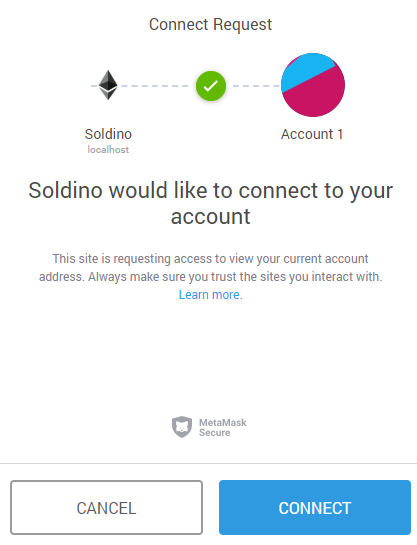
\includegraphics[width=7cm]{res/images/metamask_connect.png}
		\centering
		\caption{Connecting MetaMask to \textit{Soldino}}
	\end{figure}
	\noindent \noindent Press "Connect" and you will be redirected to a page 
	congratulating you for your registration on the platform.
	for your registration on the platform.
	\begin{figure}[H]
		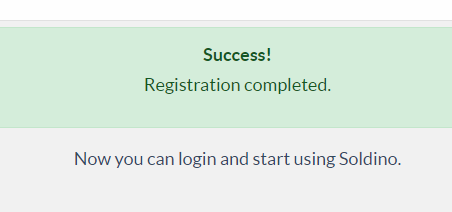
\includegraphics[width=7cm]{res/images/registration_complete.png}
		\centering
		\caption{Registration completed message}
	\end{figure}
	\subsubsection{Business is already registered}
	If your address is already registered in the platform you will see an
	error page telling you that you cannot create a new account.
	\subsection{Login}
	If you already have a business account press the "login" button on the 
	top right of the homepage. Then you will be able to buy goods and services, 
	check your orders and manage your VAT. To be able to login you have to be 
	logged in your MetaMask account.
	\subsection{Buying}
	\subsubsection{Searching}
	You can search for products by name using the search bar that can be found 
	right at the top of the page. After you start typing you will see all 
	results that match tour search. If no matching products are found you will 
	a message showing you that.
	\subsubsection{Cart}
	You can add products in your cart, after selecting the quantity you need, 
	by pressing the "Add to cart" button under it. The number on the cart shows
	you how many different products are in it.\\
	\begin{figure}[H]
		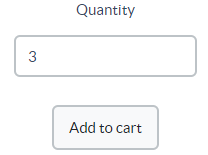
\includegraphics[width=7cm]{res/images/add_to_cart.png}
		\centering
		\caption{Adding a product to your cart}
	\end{figure}
	\noindent You can access your cart by pressing the shopping cart icon on 
	the bar at the top of the page.
	\begin{figure}[H]
		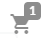
\includegraphics[width=3cm]{res/images/cart_icon.png}
		\centering
		\caption{Icon to access your cart}
	\end{figure}
	\noindent Here you will find every item you have previously selected with 
	their quantity and above them you will see the total for your order.
	If you need to modify the quantity press the "+" or "-" buttons. \\
	When you want to proceed with the order press the "Checkout" button, 
	you will be redirected to the checkout page.
	\begin{figure}[H]
		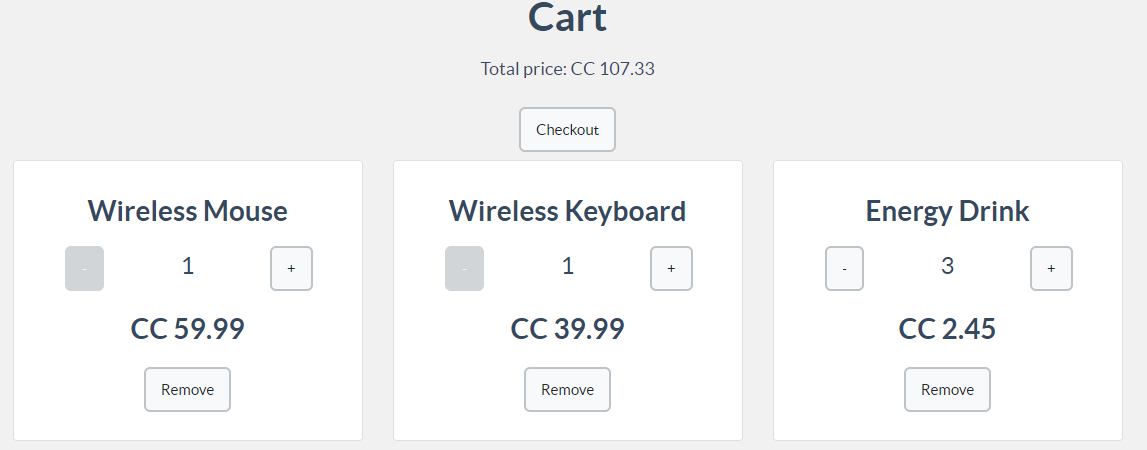
\includegraphics[width=15cm]{res/images/cart_example.png}
		\centering
		\caption{Example of content of the cart}
	\end{figure}
	\subsubsection{Checkout}
	In the checkout page you will be able to choose where your products will be 
	delivered to by using the radio buttons: you can either select the address you 
	gave during registration or enter a new one.\\
	\begin{figure}[H]
		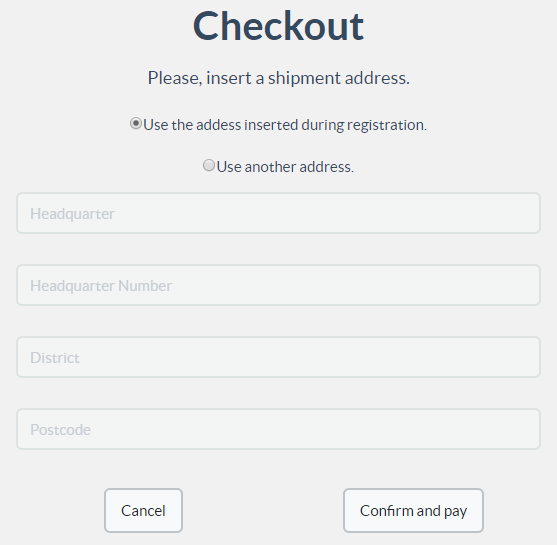
\includegraphics[width=10cm]{res/images/checkout.png}
		\centering
		\caption{Example of checkout page}
	\end{figure}
	\noindent Press the "Confirm and pay" button to proceed. In a new 
	pop up window MetaMask will ask you to confirm the transaction. The price 
	shown here will be a little higher because it includes the gas fee. \\
	Otherwise press "Cancel" to return to your cart.
	\subsubsection{Past orders}
	You can visit a the page containing all past orders by pressing the "Orders" 
	button in the bar at the top of the page.\\
	%PLACEHOLDER screen pulsante?
	Here you will find a chronological list of every purchase that you made with 
	\textit{Soldino}. Each order tells when it was made, who was the seller, 
	what were the items bought, how much you paid.
	\begin{figure}[H]
		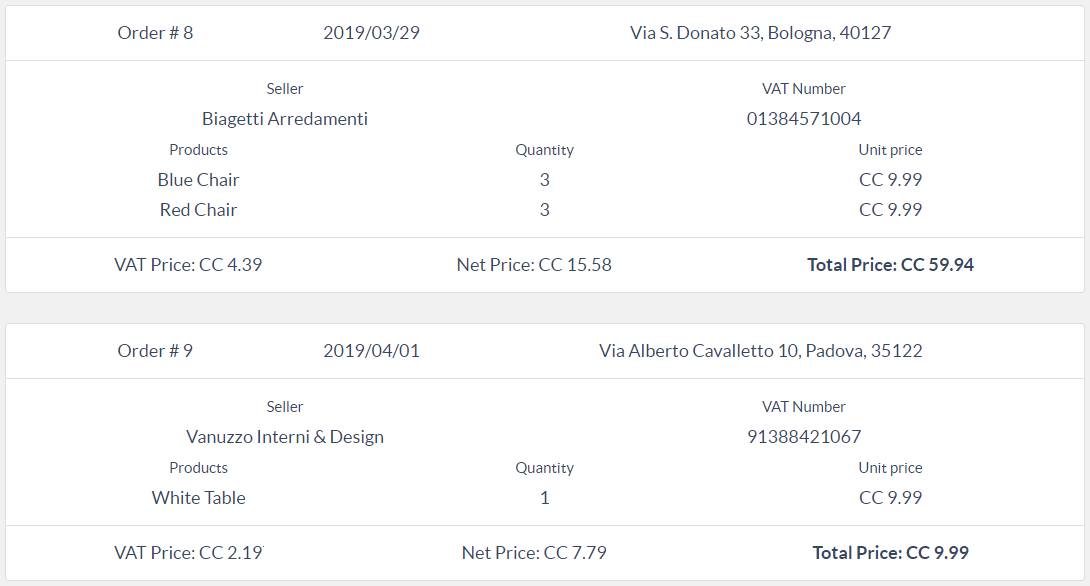
\includegraphics[width=15cm]{res/images/past_orders.png}
		\centering
		\caption{Example of past orders}
	\end{figure}

	\subsection{Selling}
	\subsubsection{Selling a new product}
	If you want to sell a new product you have to
	
	\subsubsection{Modifying a product}
	If you want to modify the information of a product you are selling you 
	have to 
	\subsubsection{Removing a product}
	If you want to remove a product from the platform you have to
	
	\subsection{VAT management}
	If you are a business \textit{Soldino} will manage VAT for the products 
	you buy and sell on the platform automatically. You can access the page 
	containing all past invoices by pressing the "Transaction Manager" button 
	on the bar at the top of the page.
	\begin{figure}[H]
		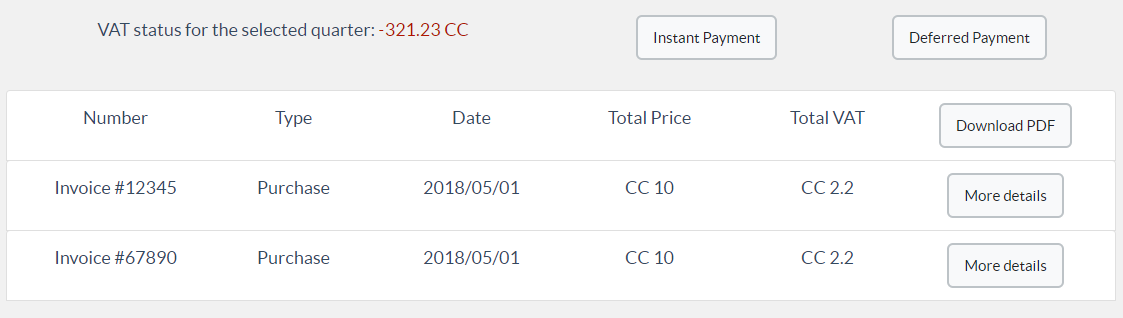
\includegraphics[width=15cm]{res/images/past_invoices.png}
		\centering
		\caption{Example of past invoices}
	\end{figure}
	\noindent You can see invoices of past trimesters by using the drop-down 
	menu at the top of the page.
	\begin{figure}[H]
		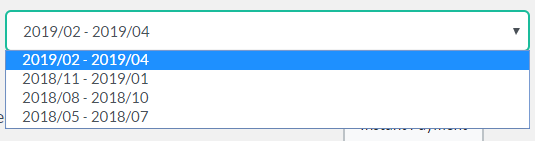
\includegraphics[width=10cm]{res/images/past_trimesters.png}
		\centering
		\caption{Past trimesters}
	\end{figure}
	
	\noindent You can see more details by pressing the "More details" button 
	on the right. This will open a pop up window containing all the details.
	\begin{figure}[H]
		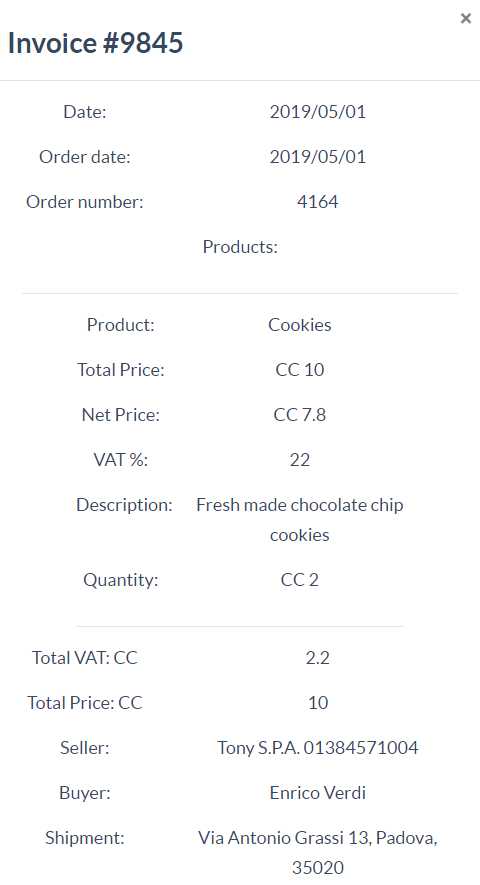
\includegraphics[width=10cm]{res/images/invoice_details.png}
		\centering
		\caption{Example of an invoice}
	\end{figure}
		\subsubsection{Paying VAT}
	
		\subsubsection{Deferring VAT}
		
		\subsubsection{Checking past trimesters' VAT}
		